% mnras_template.tex 
%
% LaTeX template for creating an MNRAS paper
%
% v3.0 released 14 May 2015
% (version numbers match those of mnras.cls)
%
% Copyright (C) Royal Astronomical Society 2015
% Authors:
% Keith T. Smith (Royal Astronomical Society)

% Change log
%
% v3.2 July 2023
%	Updated guidance on use of amssymb package
% v3.0 May 2015
%    Renamed to match the new package name
%    Version number matches mnras.cls
%    A few minor tweaks to wording
% v1.0 September 2013
%    Beta testing only - never publicly released
%    First version: a simple (ish) template for creating an MNRAS paper

%%%%%%%%%%%%%%%%%%%%%%%%%%%%%%%%%%%%%%%%%%%%%%%%%%
% Basic setup. Most papers should leave these options alone.
\documentclass[fleqn,usenatbib,openbib]{mnras}

% MNRAS is set in Times font. If you don't have this installed (most LaTeX
% installations will be fine) or prefer the old Computer Modern fonts, comment
% out the following line
\usepackage{newtxtext}
\usepackage[varvw]{newtxmath}
% Depending on your LaTeX fonts installation, you might get better results with one of these:
%\usepackage{mathptmx}
%\usepackage{txfonts}

% Use vector fonts, so it zooms properly in on-screen viewing software
% Don't change these lines unless you know what you are doing
\usepackage[T1]{fontenc}

% Allow "Thomas van Noord" and "Simon de Laguarde" and alike to be sorted by "N" and "L" etc. in the bibliography.
% Write the name in the bibliography as "\VAN{Noord}{Van}{van} Noord, Thomas"
\DeclareRobustCommand{\VAN}[3]{#2}
\let\VANthebibliography\thebibliography
\def\thebibliography{\DeclareRobustCommand{\VAN}[3]{##3}\VANthebibliography}


%%%%% AUTHORS - PLACE YOUR OWN PACKAGES HERE %%%%%

\usepackage[spanish]{babel}
\usepackage{lipsum}
\usepackage{url}
\usepackage{pgfplots}
\usepackage{booktabs, colortbl, bigstrut, multirow}

% Only include extra packages if you really need them. Avoid using amssymb if newtxmath is enabled, as these packages can cause conflicts. newtxmatch covers the same math symbols while producing a consistent Times New Roman font. Common packages are:
\usepackage{graphicx}	% Including figure files
\usepackage{amsmath}	% Advanced maths commands
\usepackage{xfrac}


\usepackage{wrapfig}
\usepackage{cuted}
\usepackage[labelfont=bf,font=footnotesize]{caption}

%%%%%%%%%%%%%%%%%%%%%%%%%%%%%%%%%%%%%%%%%%%%%%%%%%

%%%%% AUTHORS - PLACE YOUR OWN COMMANDS HERE %%%%%

\usepackage[nameinlink,noabbrev]{cleveref}
\crefformat{figure}{\textsuperscript{#2#1#3}}
\crefformat{table}{\textsuperscript{#2#1#3}}

\addto\captionsspanish{\renewcommand{\refname}{REFERENCIAS}}

\makeatletter
\def\@abstract{\list{}{%
    \listparindent\realparindent
    \itemindent\z@
    \labelwidth\z@ \labelsep\z@
    \leftmargin\z@\rightmargin\z@%%was 11pc left
    \parsep 0pt plus 1pt}\item[]%
    \reset@font\normalsize{\bf PRESENTACIÓN}\\\reset@font\abslarge
} % SFB 0.1.01
\def\@keywords{\list{}{%
    \labelwidth\z@ \labelsep\z@
    \leftmargin\z@\rightmargin\z@  %was 11pc left was 11pc\right....
    \parsep 0pt plus 1pt}\item[]\reset@font\abslarge{\bf Palabras clave: }%
}
\makeatother

\renewcommand\theequation{\Alph{equation}}

% Redefine figure environment to allow manual placement specifier
\makeatletter
\renewenvironment{figure}[1][]{%
    \@float{figure}[#1]%
}{%
    \end@float
}
\makeatother

% Redefine table environment to allow manual placement specifier
\makeatletter
\renewenvironment{table}[1][]{%
    \@float{table}[#1]%
}{%
    \end@float
}
\makeatother

% Please keep new commands to a minimum, and use \newcommand not \def to avoid
% overwriting existing commands. Example:
%\newcommand{\pcm}{\,cm$^{-2}$}	% per cm-squared

%%%%%%%%%%%%%%%%%%%%%%%%%%%%%%%%%%%%%%%%%%%%%%%%%%

%%%%%%%%%%%%%%%%%%% TITLE PAGE %%%%%%%%%%%%%%%%%%%

% Title of the paper, and the short title which is used in the headers.
% Keep the title short and informative.
\title[Medida del Índice de Refracción]{Medida del Índice de Refracción del Metacrilato y del Agua}

% The list of authors, and the short list which is used in the headers.
% If you need two or more lines of authors, add an extra line using \newauthor
\author[Álvaro Jerónimo Sánchez]{
Álvaro Jerónimo Sánchez$^{1}$, DNI: 09847051S.\thanks{E-mail: alvaro.jeronimos@estudiante.uam.es}
Copartícipe: Hugo Pérez Hernández$^{1}$
\\
% List of institutions
$^{1}$Universidad Autónoma de Madrid, Ciudad universitaria de Cantoblanco, 28049,España \\
Facultad de Ciencias, Grado en Química, FÍSICA II
}

% These dates will be filled out by the publisher
\date{Prácticas 22/04/2024. Informe 13/05/2024. Fecha Límite 16/05/2024>}

% Enter the current year, for the copyright statements etc.
\pubyear{2024}

% Don't change these lines
\begin{document}
\label{firstpage}
\pagerange{\pageref{firstpage}--\pageref{lastpage}}
\maketitle

%%%%%%%%%%%%%%%%%%%%%%%%%%%%%%%%%%%%%%%%%%%%%%%%%%

%%%%%%%%%%%%%%%%% BODY OF PAPER %%%%%%%%%%%%%%%%%%
\begin{abstract}

Se presentan medidas de los ángulos de refracción a distintos ángulos incidentes de un láser que atraviesa un medio. Se han determinado los índices de refracción de dichos medios aplicando la Ley de Snell y observando el ángulo crítico. 

\vspace{1cm}
\end{abstract}

%%%%%%%%%%%%%%%%%%%%%%%%%%%%%%%%%%%%%%%%%%%%%%%%%%
\section{Introducción Teórica}

La luz es un fenómeno que tiene un comportamiento dual. Ésta se puede definir como una onda electromagnética, lo que ayuda a describir cómo se propaga por el medio. No obstante, la energía transportada por dichas ondas se encuentra contenida (\textit{cuantizada}) en paquetes: los \textit{fotones}, hecho que implica un comportamiento corpuscular, y ayuda a comprender su emisión y absorción como corrientes de partículas. Para describir las direcciones en las que se propaga la luz, conviene representar una onda luminosa por medio de rayos (\cite{Sears}), representando estos o bien la trayectoria de las partículas (comportamiento corpuscular), o bien la línea por la que se propaga la onda (comportamiento ondulatorio). Para estudiar la reflexión y refracción de la luz, se empleará este modelo. 

Un láser es una fuente que induce a los átomos a emitir luz de forma coherente, consiguiendo un haz de luz concentrado, de alta intensidad y prácticamente monocromático. Cuando éste incide en un material transparente, puede ser reflejado y refractado parcialmente (a través del material hasta volver a salir al medio inicial). El láser incide con un ángulo sobre la normal de la superficie denominado \textit{ángulo incidente}, y saldrá describiendo otro al que llamamos \textit{ángulo refractado}. En el caso de que también se produzca reflexión, habrá también un \textit{ángulo reflejado}. 

El índice de refracción ($n$) de un material relaciona la velocidad de la luz en el vacío ($c$) y en el material ($v$) con la fórmula: $n=\frac{c}{v}$. En el vacío $n=1$, pero en cualquier otro medio será mayor, ya que la luz viajará más lentamente ($v<c$). La \textit{ley de Snell} relaciona los índices de un par de materiales con el ángulo de incidencia y el reflejado:
\begin{gather}
    n\sin\Phi = n'\sin\Phi' \label{eq:snell}
\end{gather}
El ángulo crítico es el ángulo de incidencia para el cual el rayo refractado emerge tangente a la superficie, produciéndose una reflexión. Todos los ángulos mayores a éste producirán reflexión. Al ser tangente, $\Phi=90^{\circ}$, por lo que, sustituyendo en la ley de Snell (\ref{eq:snell}) obtenemos:
\begin{gather}
    \sin\Phi_{crit}=\frac{n}{n'} \label{eq:crit}
\end{gather}

%%%%%%%%%%%%%%%%%%%%%%%%%%%%%%%%%%%%%%%%%%%%%%%%%%
\section{Montaje experimental}

\subsection{Material empleado}

Para las medidas de los ángulos se ha empleado una plataforma giratoria en la que se indican grados con un error de $\pm 1^{\circ}$. El láser empleado es un láser de diodo de 635 nm y potencia $<$1 mW. Los materiales a estudiar han sido un sólido semicircular de metacrilato (PMMA) y agua de grifo, empleando una cubeta semicircular de plástico (que prácticamente no variaba la trayectoria) para contenerla.

\subsection{Medición}

El proceso de toma de medidas ha sido el mismo para ambos materiales. Primero se ha posicionado el láser en el \textit{0} de la plataforma. Se ha situado el semicírculo (sea la cubeta con agua o el sólido) en la línea marcada en la plataforma de forma perpendicular al láser, de forma que éste incidiese sobre la cara plana. Se ha ido rotando la plataforma de grado en grado, tomando medidas del ángulo refractado a distintos ángulos incidentes entre 0 y 70 grados. Tras haber realizado estas medidas, se ha ido lentamente buscando (en cada material) el punto en el que se producía una reflexión tangente a la superficie, y se ha notado su ángulo incidente como el ángulo crítico.

%%%%%%%%%%%%%%%%%%%%%%%%%%%%%%%%%%%%%%%%%%%%%%%%%%
\section{Cálculos}

Una vez tomadas las medidas, se han calculado los senos de los ángulos $\Phi$ y $\Phi'$ para posteriormente graficarlos. En este caso, la pendiente de la gráfica correspondería a $\frac{\sin\Phi}{\sin\Phi'}$, que es equivalente a $\frac{n'}{n}$, aplicando Snell (\ref{eq:snell}). Al ser el índice de refracción del aire $\approxeq 1$, la pendiente será aproximadamente igual al índice de refracción del material estudiado. 

Se han comparado estos resultados con los obtenidos aplicando la expresión del ángulo crítico (\ref{eq:crit}) para cada material.

\subsection{Errores}

\begin{table*} %this is a figure from "Resultados"
    \centering
    \caption{Tablas de medidas cogidas para ambos materiales con sus respectivos errores.}
    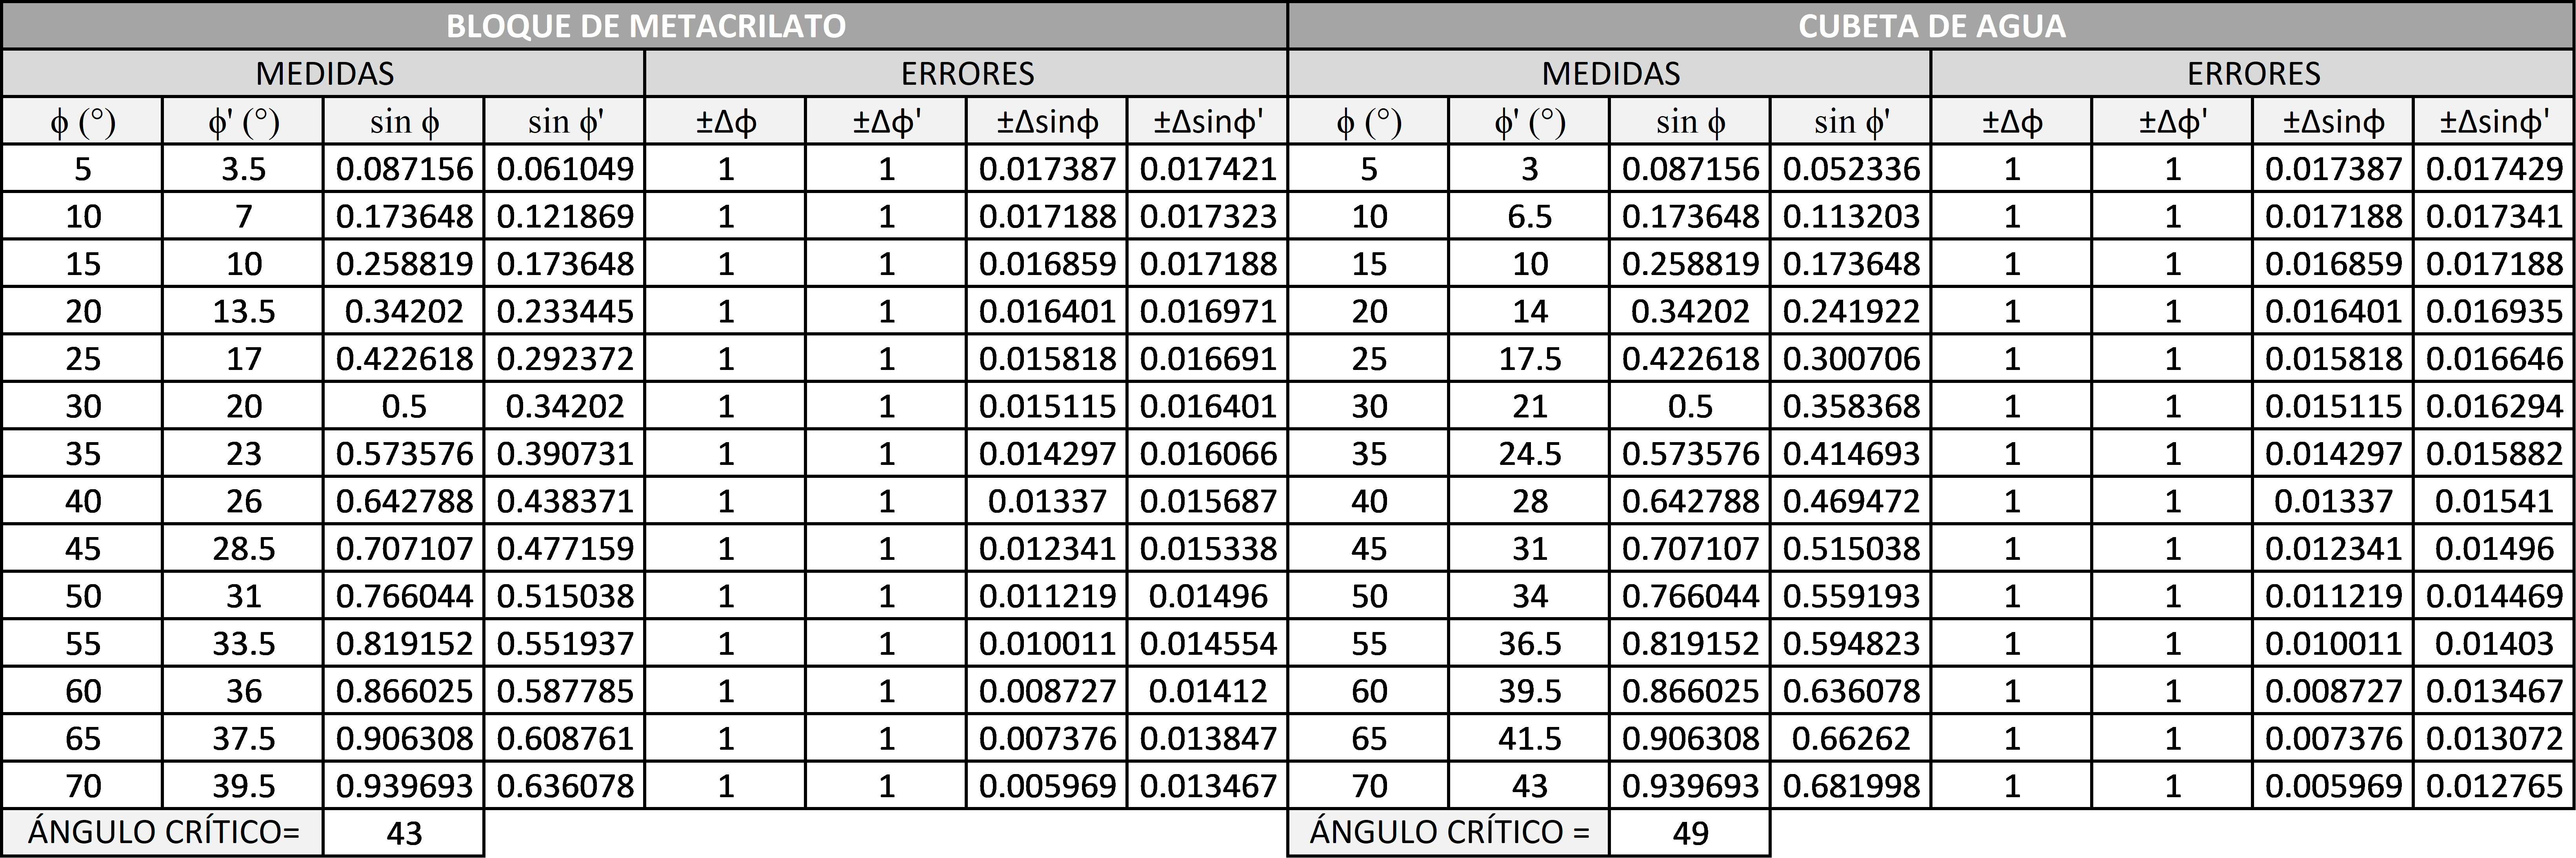
\includegraphics[width=0.9\textwidth]{images/tables.png}
    \label{tab:tables}
\end{table*}

El error de los ángulos es siempre $\pm 1^{\circ}$, ya que corresponde con el error de la plataforma giratoria. Para calcular los errores de los senos, se deriva la expresión y se realiza propagación de errores (con los ángulos convertidos a radianes), obteniendo:
\begin{gather*}
    \Delta \sin\Phi = \cos\Phi\cdot\Delta\Phi
\end{gather*}
Para hallar el error de las pendientes de las rectas (que corresponde con los índices de refracción ''$n$'') que se ha calculado por mínimos cuadrados con \textit{Excel}, se ha usado la función \textit{ESTIMACION.LINEAL} (ver sección \ref{resultados}).

El error de los resultados provenientes de la expresión del ángulo crítico (\ref{eq:crit}) se ha obtenido por propagación, teniendo que haber convertido grados a radianes:
\begin{gather*}
    \sin\Phi_{crit}=\frac{n}{n'}=\frac{1}{n'}\implies n'=\frac{1}{\sin\Phi_{crit}}\\
    \implies \Delta n' = \frac{\partial \sin^{-1}\Phi_{crit}}{\partial n'}\Delta\Phi = \frac{\cos\Phi}{\sin^2\Phi}\Delta\Phi
\end{gather*}

\subsection{Resultados}
\label{resultados}

\textit{(Medidas y resultados en Tabla \ref{tab:tables}).}

Tras realizar los cálculos con la expresión del ángulo crítico \ref{eq:crit}, se han obtenido datos muy similares a los hallados con las pendientes:

\begin{table}[h]
    \centering
    \begin{tabular}{ccc}
        \hline
        Cálculo & Metacrilato & Agua \\
        \hline
        \textbf{Pendientes} & $1.49\pm 0.0062$ & $1.34\pm 0.0052$ \\
        \textbf{Snell} & $1.47\pm 0.027$ & $1.33\pm 0.020$ \\
        \hline
    \end{tabular}
\end{table}

%%%%%%%%%%%%%%%%%%%%%%%%%%%%%%%%%%%%%%%%%%%%%%%%%%
\section{Conclusión}

Con estos resultados se puede concluir que se cumple la ley de Snell (\ref{eq:snell}) y los datos experimentales son correctos. Se puede observar cómo el metacrilato posee mayor índice de refracción que el agua, es decir, la luz viaja más lenta a través de éste. Esto puede ser debido a que la densidad del metacrilato es mayor, y la velocidad de la luz tiende a disminuir (el índice de refracción aumenta) cuanto mayor es la densidad del material (\cite{cant}). La densidad del agua es de $\approxeq 1 g/cm^3$, mientras que la del metacrilato es de $\approxeq 1.18 g/cm^3$, lo que corrobora lo hallado.

\begin{figure}[h]
    \centering
    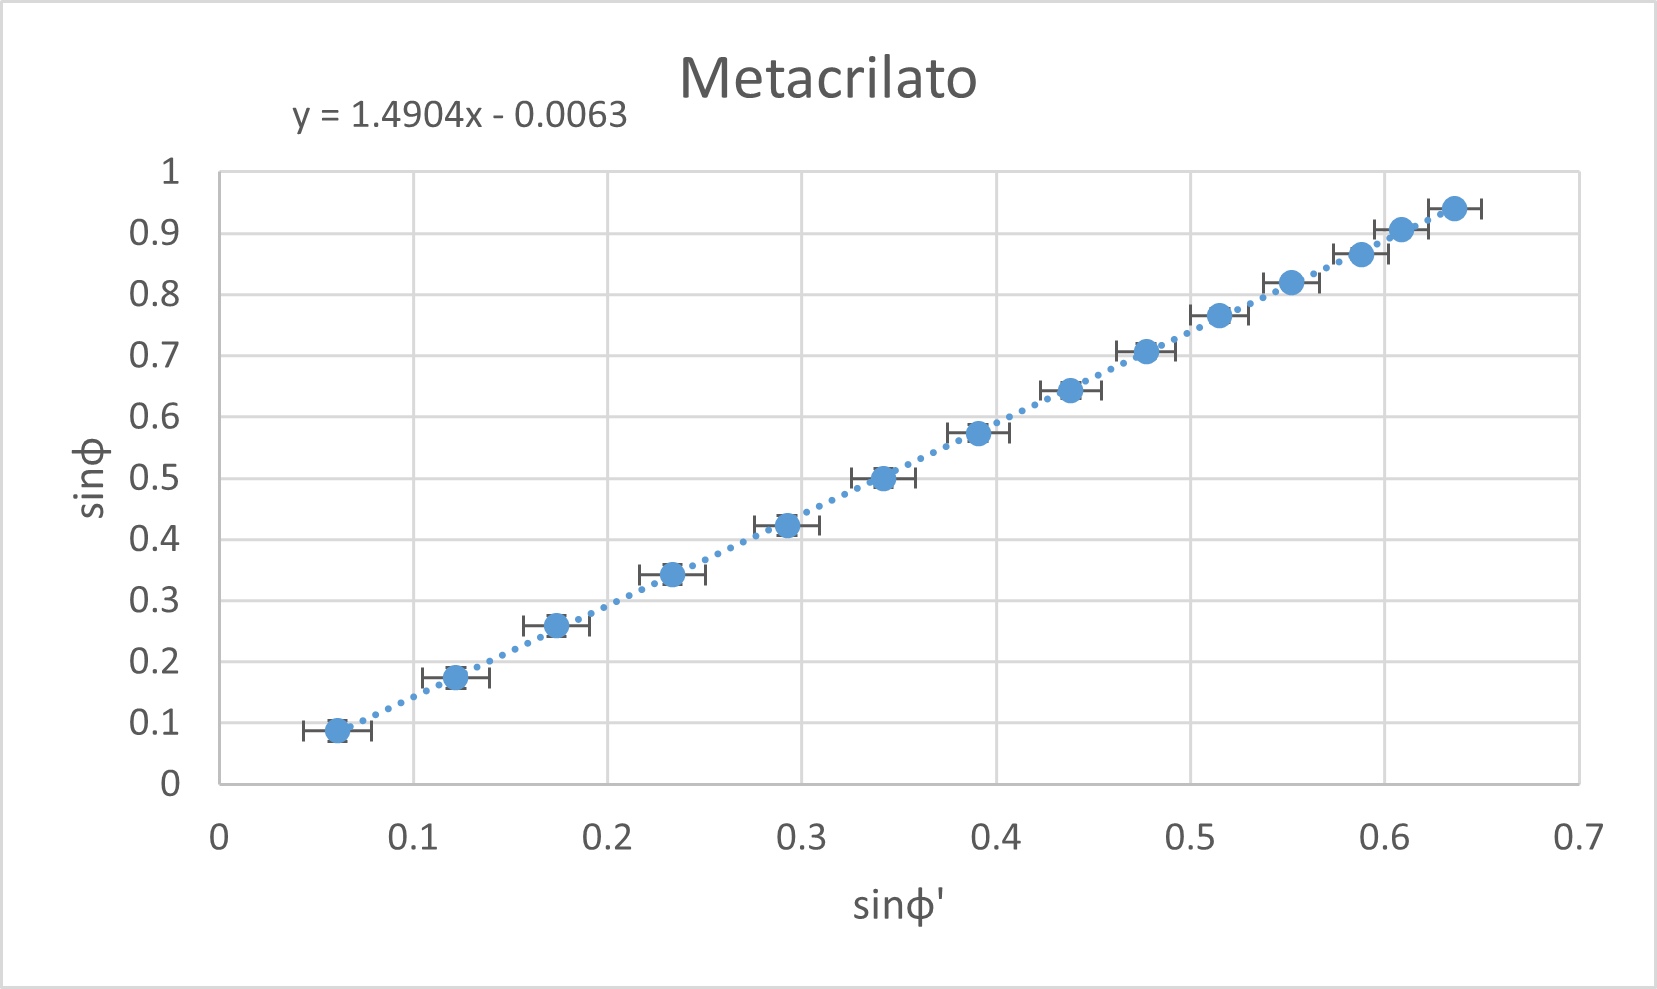
\includegraphics[width=0.9\columnwidth]{images/metacrilato.png}
    \caption{Gráfica $\sin\Phi-\sin\Phi'$ del metacrilato}
    \label{fig:metacrilato}
\end{figure}

\begin{figure}[h]
    \centering
    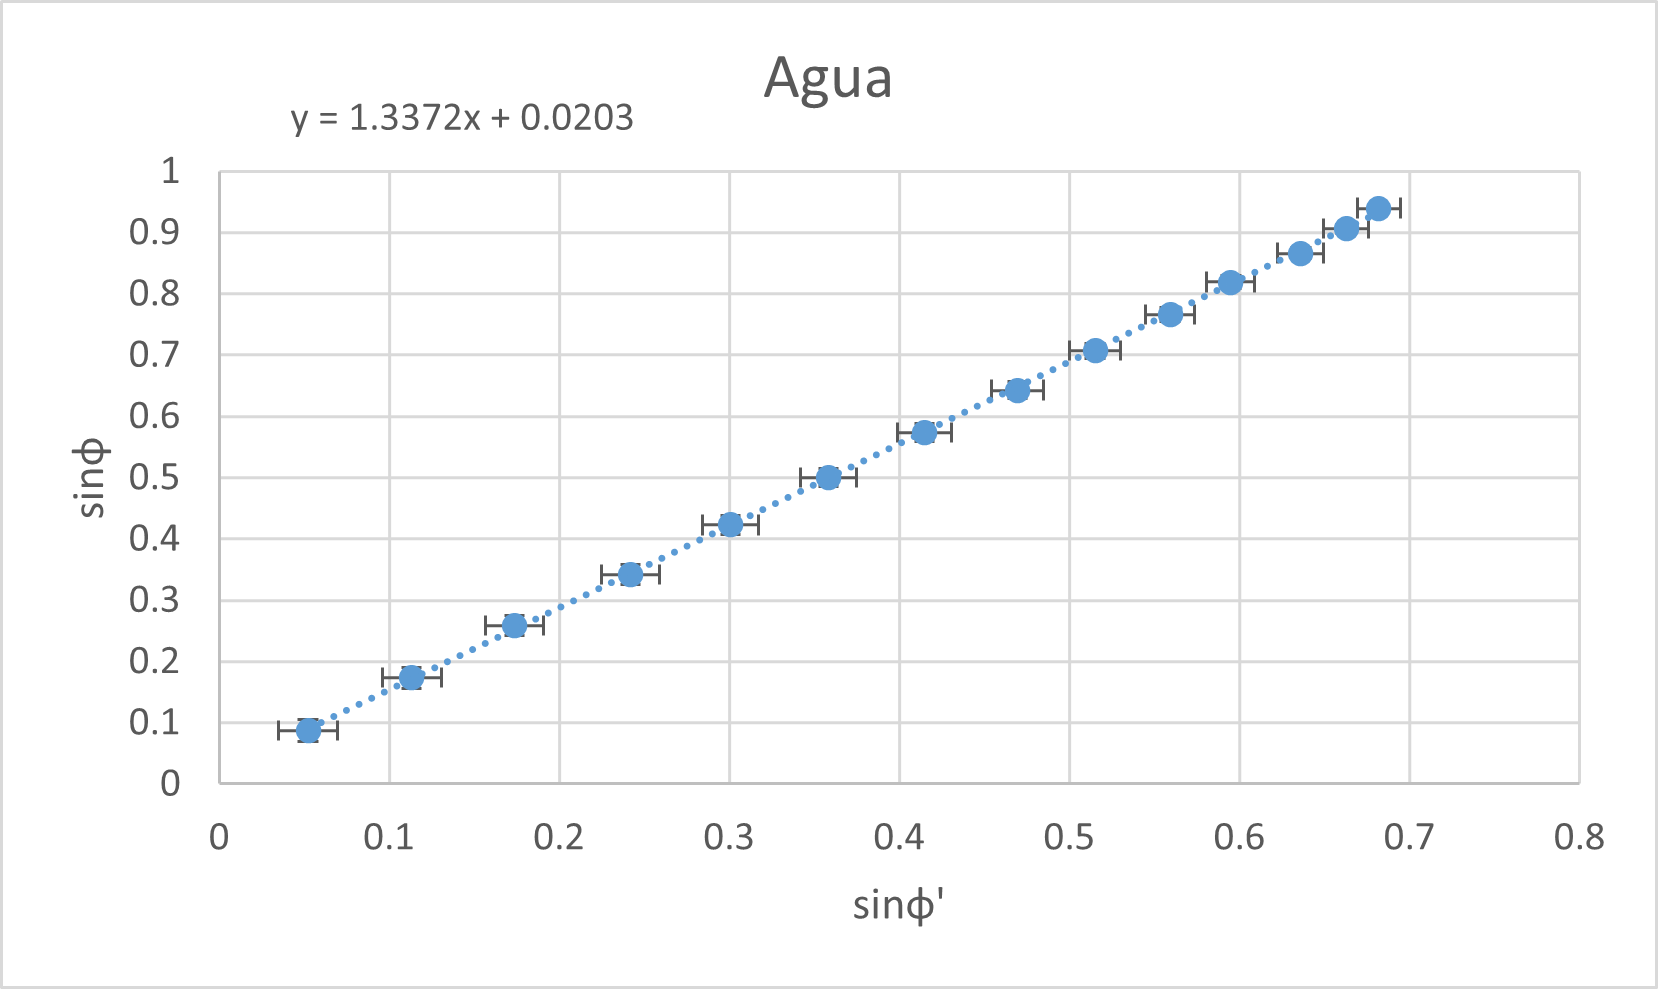
\includegraphics[width=0.9\columnwidth]{images/agua.png}
    \caption{Gráfica $\sin\Phi-\sin\Phi'$ del agua}
    \label{fig:agua}
\end{figure}

    \captionof{figure}{Gráfica a mano en papel milimetrado $\sin\Phi'$-$\sin\Phi$ del metacrilato}
\textit{(Gráficas a mano en el apéndice [\ref{appendix}])}

%%%%%%%%%%%%%%%%%%%% REFERENCES %%%%%%%%%%%%%%%%%%

% The best way to enter references is to use BibTeX:
\vfill
\nocite{*}
\bibliographystyle{mnras}
\bibliography{bibliography}


% Alternatively you could enter them by hand, like this:
% This method is tedious and prone to error if you have lots of references
%\begin{thebibliography}{99}
%\bibitem[\protect\citeauthoryear{Author}{2012}]{Author2012}
%Author A.~N., 2013, Journal of Improbable Astronomy, 1, 1
%\bibitem[\protect\citeauthoryear{Others}{2013}]{Others2013}
%Others S., 2012, Journal of Interesting Stuff, 17, 198
%\end{thebibliography}

%%%%%%%%%%%%%%%%%%%%%%%%%%%%%%%%%%%%%%%%%%%%%%%%%%

%%%%%%%%%%%%%%%%% APPENDICES %%%%%%%%%%%%%%%%%%%%%
\clearpage
\appendix

\begin{strip}
    \section*{Apéndice}
    \label{appendix}
    \centering
    
    \captionof{figure}{Gráfica a mano en papel milimetrado $\sin\Phi'$-$\sin\Phi$ del metacrilato}
    \includegraphics[width=0.7\linewidth]{images/hand-metacrilato.png}
    
    \centering
    
    \captionof{figure}{Gráfica a mano en papel milimetrado $\sin\Phi'$-$\sin\Phi$ del agua}
    \includegraphics[width=0.7\linewidth]{images/hand-agua.png}
    
    \end{strip}

%%%%%%%%%%%%%%%%%%%%%%%%%%%%%%%%%%%%%%%%%%%%%%%%%%


% Don't change these lines
\bsp	% typesetting comment
\label{lastpage}
\end{document}

% End of mnras_template.tex